\chapter{ROLLO: Reactor evOLutionary aLgorithm Optimizer}
\label{chap:rollo}
% todo: need a nice rollo v1.0 citation
In this chapter, I introduce the \gls{ROLLO} framework developed for this dissertation. 
\gls{ROLLO} is a Python package that applies evolutionary algorithm 
techniques to optimize nuclear reactor design. 
Applying evolutionary algorithms to nuclear design problems is not new, as
discussed in Section \ref{sec:opt}. 
Reactor designers have individually customized available evolutionary algorithm 
packages for their reactor design optimization problems.
However, the evolutionary algorithm setup is highly customizable with
an assortment of genetic algorithm designs and related operators.
A reactor designer unfamiliar with evolutionary algorithms will have
to go through the cumbersome process of customizing a genetic algorithm 
for their needs and determine which operators and hyperparameters work best for 
their problem. 
Furthermore, computing fitness values with nuclear software is computationally 
expensive, necessitating using supercomputers. 
Reactor designers have to set up parallelization to use the genetic algorithm 
in concert with nuclear software.

Therefore, the motivation for \gls{ROLLO} is to limit these inconveniences and 
facilitate using evolutionary algorithms for reactor design optimization.
\gls{ROLLO} provides a general genetic algorithm framework, sets up 
parallelization for the user, and promotes usability with an input file 
that only exposes mandatory parameters.
\gls{ROLLO} strives to be effective, flexible, open-source, parallel, reproducible, 
and usable. 
I briefly summarize how \gls{ROLLO} achieves these goals:
\begin{itemize}
    \item Effective: \gls{ROLLO} is well documented and tested.
    \item Flexible: This dissertation uses \gls{ROLLO} to 
    explore arbitrary reactor geometries and heterogeneous fuel distributions. 
    However, future users might want to utilize \gls{ROLLO} 
    to explore other arbitrary design parameters. Thus, I designed the \gls{ROLLO}
    framework accordingly. The user can vary any imaginable parameter 
    because \gls{ROLLO} uses a templating method to edit the input file of the 
    coupled software.
    \item Open-source: \gls{ROLLO} is version-controlled on Github 
    \cite{chee_rollo_2021}. \gls{ROLLO} also utilizes the well-documented, open-source 
    \gls{DEAP} \cite{fortin_deap_2012} Python package to drive the evolutionary 
    algorithm optimization process.
    % todo: add sentence saying why open source helps your code too. 
    \item Parallel: Users have the option to run \gls{ROLLO} in parallel so that 
    they may effectively use the computational resources available. 
    \item Reproducible: Data from every \gls{ROLLO} run saves into a unique, pickled 
    checkpoint file (pickle is a Python module that serializes Python objects). 
    The checkpoint file contains the \gls{ROLLO} input file and coupled evaluator's 
    scripts enabling results replication. The checkpoint file also acts as a restart 
    file for partially completed simulations. 
\end{itemize}

\gls{ROLLO} provides a framework to couple an evolutionary algorithm driver with nuclear 
software, such as neutron transport and thermal-hydraulics codes. 
\gls{ROLLO} is nuclear code-agnostic and does not have any hard dependencies on any 
nuclear software. 
Figure \ref{fig:genetic_alg} from Chapter \ref{chap:lit-review} outlined a
general evolutionary algorithm iterative problem solving process. 
I modified Figure \ref{fig:genetic_alg} to produce Figure 
\ref{fig:genetic_alg_nuclear}, which depicts how the nuclear transport and 
thermal-hydraulics software fit within \gls{ROLLO}'s evolutionary algorithm 
optimization process. 
% need to update with new algorithm style
\begin{figure}[htbp]
    \centering
    \begin{tikzpicture}[node distance=1.7cm]
            \tikzstyle{every node}=[font=\small]
            \node (1) [lbblock] {\textbf{Create initial population}};
            \node (2) [loblock, below of=1] {\textbf{Evaluate initial population}};
            \node (3) [lbblock, below of=2, yshift = -1.3cm] {\textbf{Create offspring population:} \\ 
            \begin{enumerate} \item Apply \textbf{crossover} operator to previous population
                              \item Apply \textbf{mutation} operator to previous population
                              \end{enumerate}};
            \node (4) [loblock, below of=3, yshift=-1.3cm] {\textbf{Evaluate offspring population}};
            \node (7) [lbblock, below of=4, yshift = -1.3cm] {\textbf{Create new population:} \\
            \begin{enumerate} \item Apply \textbf{selection} operator to offspring + previous population
                              \item Apply constraints to new population
                              \end{enumerate}};
            \node (5) [lbblock, below of=7, yshift=-1.3cm] {\textbf{Is termination \\ criteria satisfied?}};
            \node (6) [lbblock, below of=5] {\textbf{Best solution is returned!}};
            \draw [arrow] (1) -- (2);
            \draw [arrow] (2) -- (3);
            \draw [arrow] (3) -- (4);
            \draw [arrow] (4) -- (7);
            \draw [arrow] (7) -- (5);
            \draw [arrow] (5) -- node[anchor=east] {yes} (6);
            \draw [arrow] (5) -- ([shift={(0.5cm,0cm)}]5.east)-- node[anchor=west] {no} ([shift={(0.5cm,0cm)}]3.east)--(3);
            \matrix [draw,above right,yshift=10.7cm, xshift=0cm] at (current bounding box.south east) {
            \node [bbblock,label=right:\textbf{EA: Evolutionary Algorithm}] {}; \\
            \node [boblock,label=right:\textbf{NS: Nuclear Software}] {}; \\
            };
    \end{tikzpicture}
    \caption{Process of finding optimal solutions for a problem with a 
    genetic algorithm. Nuclear software evaluates each new population.}
    \label{fig:genetic_alg_nuclear}
\end{figure}
\gls{ROLLO} initially reads and validates the JSON input 
file, initializes the \gls{DEAP} \cite{fortin_deap_2012} genetic algorithm 
hyperparameters and operators, and finally runs the genetic algorithm following 
the flow chart in Figure \ref{fig:genetic_alg_nuclear}, in which the nuclear 
software evaluates each individual reactor model's fitness. 

The subsequent sections describe \gls{ROLLO}'s evolutionary algorithm driver 
software \gls{DEAP} (Section \ref{sec:rollo-ea}), input file structure (Section 
\ref{sec:rollo-input-file}), software architecture (Section \ref{sec:rollo-archi}), 
verification studies (Section \ref{sec:rollo-verification}), and convergence criteria
(Section \ref{sec:rollo-convergence}). 
Appendix B lists all the data and analysis related to this chapter to enable the 
reproduction of all the simulations.

\section{Evolutionary Algorithm Driver}
\label{sec:rollo-ea}
Evolutionary algorithm computation uses sophisticated, diverse techniques 
and mechanisms, resulting in even the most well-designed software frameworks 
being complicated under the hood. 
Utilizing an existing evolutionary algorithm framework presents implementation 
challenges as the user must edit the framework's source code to customize it for their 
application and hyperparameters \cite{fortin_deap_2012}. 
Therefore, a computation framework that gives the user the capability to build 
custom evolutionary algorithms is ideal for this project.

Many evolutionary algorithm computation packages exist: 
\gls{DEAP} \cite{fortin_deap_2012}, Pymoo \cite{blank_pymoo_2020}, inspyred 
\cite{garrett_inspyred_2014}, Pyevolve \cite{perone_pyevolve_2009}, and 
OpenBEAGLE \cite{gagne_open_2002}.
\gls{DEAP} is the newest package and places a high value on code 
compactness and clarity \cite{fortin_deap_2012}. 
\gls{DEAP} is the only framework that allows the user to prototype evolutionary 
algorithms rapidly and define custom algorithms without digging deep into 
the source code to modify hyperparameters and their application methods.
Accordingly, I chose \gls{DEAP} to drive the \gls{ROLLO} framework's 
evolutionary algorithm component. 
\gls{DEAP} provides building blocks for each optimizer function and allows the 
user to customize a specialized algorithm to fit their project \cite{fortin_deap_2012}.

\subsection{Distributed Evolutionary Algorithms in Python}
\label{sec:deap-works}
\gls{DEAP} is composed of two structures: a \textit{creator} and a 
\textit{toolbox}.  
The \textit{creator} module allows the run-time creation of classes via 
inheritance and composition, enabling individual and population creation 
from any data structure: lists, sets, dictionaries, trees, etc \cite{fortin_deap_2012}. 
The \textit{toolbox} is a container that the user manually populates.
In the \textit{toolbox}, the user defines the selection, crossover, and 
mutation operator types and their respective hyperparameters.
For example, the user registers a crossover operator under the `mate'
alias and a selection operator under the `select' alias. 
Then, the evolutionary algorithm uses these aliased operators from the 
\textit{toolbox}. 
If the user wants to change the crossover operator, they update the 
`mate' alias in the \textit{toolbox} while keeping the evolutionary algorithm 
unchanged \cite{fortin_deap_2012}. 

Figure \ref{fig:deap-code} illustrates \gls{DEAP}'s usage of the \textit{creator} and
\textit{toolbox} modules. 
\begin{figure}[htbp]
    \begin{minted}[
        frame=lines,
        framesep=2mm,
        baselinestretch=1.2,
        fontsize=\footnotesize,
        linenos
        ]{python}
        
        from deap import creator, base, tools, algorithms
        creator.create("Objective", base.Fitness, weights=(-1.0,)) # minimum
        creator.create("Individual", list, fitness=creator.Objective)

        toolbox = base.Toolbox()
        toolbox.register("variable_1", random.uniform, 0.0, 10.0)
        toolbox.register("variable_2", random.uniform, -1.0, 0.0)
        def individual_creator():
            return creator.Individual([toolbox.variable_1(), toolbox.variable_2()])
        toolbox.register("individual", individual_creator())
        toolbox.register("population", tools.initRepeat, list, toolbox.individual)
        def evaluator_fn(individual):
            return tuple([sum(individual)])
        toolbox.register("evaluate", evaluator_fn)
        toolbox.register("select", tools.selBest, k=5)
        toolbox.register("mutate", tools.mutPolynomialBounded, eta=0.5, low=[0, -1], up=[-1, 0])
        toolbox.register("mate", tools.cxOnePoint)
    \end{minted}
    \caption{DEAP sample code demonstrating the usage of the \textit{creator} and
    \textit{toolbox} modules to initialize the genetic algorithm. In \gls{ROLLO}, \gls{DEAP}'s 
    \textit{creator} and \textit{toolbox} modules are initialized in the source 
    code based on the genetic algorithm parameters defined by the user in the 
    \gls{ROLLO} input file. }
    \label{fig:deap-code}
\end{figure}
Line 2 creates a single-objective fitness class, \texttt{Objective}. 
The first argument defines the derived class's name; the second argument 
specifies the inherited base class, \texttt{base.fitness}; the third 
argument indicates the objective fitness ($-1.0$ indicates a minimum objective, 
$+1.0$ indicates a maximum objective). 
Line 3 derives an \texttt{Individual} class from the standard Python list type
and defines its fitness attribute as the newly created \texttt{Objective} object. 
Lines 5-9 initialize the \gls{DEAP} toolbox, register 
\texttt{variable\_1} and \texttt{variable\_2} with their upper and lower bounds, 
and defines the \texttt{individual\_creator} function to return an 
\texttt{Individual} initialized with \texttt{variable\_1} and \texttt{variable\_2}. 
Lines 10-11 and 14-17 are aliases for initializing individuals and populations, 
specifying variation operators (\texttt{select}, \texttt{mutate}, \texttt{mate}), 
and evaluating individual fitness (\texttt{evaluate}) \cite{fortin_deap_2012}. 
Lines 12-13 define the evaluation function that returns the fitness values. 

\gls{ROLLO} initializes \gls{DEAP}'s \textit{creator} and \textit{toolbox} modules 
based on the genetic algorithm parameters defined by the user in the \gls{ROLLO} 
input file. 
The evaluation function runs the nuclear software and returns user-defined 
fitness values. 

\subsection{ROLLO Evolutionary Algorithm Implementation}
\gls{DEAP} creators provided variations of a classical genetic algorithm 
exposing different explicitness levels \cite{fortin_deap_2012}. 
The high-level examples use the built-in \gls{DEAP} genetic algorithms, 
whereas the low-level example completely unpacks the genetic algorithm to expose 
a generational loop. 
I included an unpacked genetic algorithm in ROLLO's 
\textbf{\textit{Algorithm}} class, depicted in Figure \ref{fig:genetic_alg_nuclear}. 
The algorithm begins by initializing the starting population and evaluating 
each individual's fitness value. 
Then, it enters a generational loop. 
During each iteration, the mating and mutation operators are applied to the population
to create an offspring population, and all offspring individuals are evaluated. 
The selection operator is then applied to both the previous and offspring populations 
to select the best individuals to create the new population. 
Finally, the constraints are applied, and the results are saved.
Applying the selection operator to the combined previous and offspring 
populations expands the population, ensuring the effectiveness of 
elitism selection operators, such as NSGA-II, which work well 
for multiobjective optimization. 

\section{ROLLO Input File}
\label{sec:rollo-input-file}
\gls{ROLLO}'s input file is in JSON format. 
There are four sections that the user must define: \\ \texttt{control\_variables}, 
\texttt{evaluators}, \texttt{constraints}, and \texttt{algorithm}. 
Figure \ref{fig:rollo-input} shows an example \gls{ROLLO} input file. 
In this example, \gls{ROLLO} uses a genetic algorithm with user-defined 
hyperparameters, defined in the \texttt{algorithm} secion, to minimize the 
\texttt{output1} parameter.
The OpenMC evaluator accepts input parameters: \texttt{variable1} and 
\texttt{variable2}, and calculates the \texttt{output1} parameter.
\begin{figure}[htbp]
    \begin{minted}[
        frame=lines,
        framesep=2mm,
        baselinestretch=1.2,
        fontsize=\footnotesize,
        linenos
        ]{json}
        {
            "control_variables": {
                "variable1": {"min": 0.0, "max": 10.0}, 
                "variable2": {"min": -1.0, "max": 0.0}
            }, 
            "evaluators": {
                "openmc": {
                    "order": 0,
                    "inputs": ["variable1", "variable2"],
                    "input_script": ["python", "openmc_inp.py"],
                    "execute": [["openmc"],],
                    "outputs": ["output1", "output2"]
                    "output_script": ["python", "openmc_output.py"], 
                }
            }, 
            "constraints": {
                "output1": {"operator": [">=", "<"], "constrained_val": [1.0, 1.5]}
            }, 
            "algorithm": {
                "objective": ["min"], 
                "weight": [1.0],
                "optimized_variable": ["output1"], 
                "pop_size": 100, 
                "generations": 10, 
                "parallel": "job_control",
                "keep_files": "all",
                "mutation_probability": 0.23,
                "mating_probability": 0.46,
                "selection_operator": {"operator": "selTournament", "tournsize":5},
                "mutation_operator": {
                    "operator": "mutPolynomialBounded",
                    "indpb": 0.23,
                    "eta": 0.23
                },
                "mating_operator": {"operator": "cxBlend", "alpha": 0.46}
            }
        }
    \end{minted}
    \caption{\acrfull{ROLLO} sample JSON input file.}
    \label{fig:rollo-input}
\end{figure}
Next, I describe how to define each section of a \gls{ROLLO} input file. 
The \gls{ROLLO} documentation \cite{chee_documentation_2021} provides further 
descriptions for setting up a \gls{ROLLO} input file.

\subsection{Control Variables}
I use the term control variables to refer to parameters the genetic algorithm will 
vary (conventionally, a control variable is held constant in a research study 
however this is not the case for \gls{ROLLO}).
The user must specify the minimum and maximum values for each control variable.
For example, Lines 2 to 5 in Figure \ref{fig:rollo-input} demonstrate that the 
control variables, \texttt{variable1} and \texttt{variable2}, 
will be varied from 0 to 10 and -1 to 0, respectively. 
For example, in traditional reactor design, a control variable might be fuel 
enrichment. 

\subsection{Evaluators}
Evaluators are the nuclear software \gls{ROLLO} utilizes to calculate objective functions. 
\gls{ROLLO} is nuclear code-agnostic and does not have hard dependencies on any 
nuclear software.
Thus, it is up to the user to ensure that the nuclear software and their corresponding 
executables are correctly installed. 
In a single \gls{ROLLO} input file, users may define any number of evaluators. 
For each evaluator, mandatory parameters are \texttt{order}, \texttt{input\_script}, 
\texttt{inputs}, and \texttt{outputs}, and the optional parameters are
\texttt{execute} and \texttt{output\_script}. 
Table \ref{tab:evaluator-inputs} describes each evaluator's mandatory and optional parameters 
in the \gls{ROLLO} \texttt{evaluators}' input file section.  
\begin{table}[htbp]
    \centering
    \onehalfspacing
    \caption{\acrfull{ROLLO} \texttt{evaluator}: Input Parameter Descriptions.}
	\label{tab:evaluator-inputs}
    \footnotesize
    \begin{tabular}{l|lp{2.5cm}p{7cm}}
    \hline
    & \textbf{Parameter} & \textbf{Type} & \textbf{Description} \\
    \hline
    \multirow{9}{2cm}{Mandatory Parameters} & \texttt{order} & int 
    & evaluator's operational order compared to other evaluators (indexed by 0) \\
    \cline{2-4}
    & \texttt{inputs} & list of strings & control variables to be placed in the input 
    script template \\
    \cline{2-4}
    & \texttt{input\_script} & list of strings (2-element) & 1st element: executable to 
    run input script, 2nd element: input script template \\
    \cline{2-4}
    & \texttt{outputs} & list of strings & output variables that the evaluator will return to the genetic algorithm \\
    \hline
    \multirow{4}{2cm}{Optional Parameters} & \texttt{execute} & list of 2-element lists &
    enables users to run other executables or files beyond the input and output scripts. 
    1st element: executable to run file, 2nd element: file to run \\
    \cline{2-4}
    & \texttt{output\_script} & list of strings (2-element) & 1st element: executable to 
    run output script, 2nd element: output script template \\
    \hline 
    \end{tabular}
    \end{table}

\gls{ROLLO} utilizes jinja2 templating \cite{ronacher_welcome_2018} to insert 
the control variable values into the \texttt{input\_script}.
Users must include each evaluator's input file template in the same directory as the \gls{ROLLO} input 
file. 
Users must also ensure the template variables correspond to the \texttt{inputs} defined in the 
corresponding evaluator's section in the ROLLO input file. 
Lines 6 to 13 in the \gls{ROLLO} input file (Figure \ref{fig:rollo-input}) demonstrate 
that \texttt{variable1} and \texttt{variable2} are \texttt{inputs} into the 
\texttt{openmc\_inp.py} \texttt{input\_script}. 
Figure \ref{fig:openmcinp.py} shows the template and templated openmc script; 
once the \texttt{openmc\_inp.py} \texttt{input\_script} is templated, 
\texttt{\{\{variable1\}\}} and \texttt{\{\{variable2\}\}}  on Lines 3 and 4 will be 
replaced with values selected by the \gls{ROLLO} genetic algorithm. 
\begin{figure}[htbp]
    \begin{minipage}{0.4\textwidth}
        \centering
    \begin{minted}[
        frame=lines,
        framesep=2mm,
        baselinestretch=1.2,
        fontsize=\footnotesize,
        linenos
        ]{python}
        import openmc 
        # templating 
        variable1 = {{variable1}}
        variable2 = {{variable2}}
        # run openmc 
        ... 
    \end{minted}
    \end{minipage}
    \hspace{2cm}
    \begin{minipage}{0.4\textwidth}
        \centering
        \begin{minted}[
            frame=lines,
            framesep=2mm,
            baselinestretch=1.2,
            fontsize=\footnotesize,
            linenos
            ]{python}
            import openmc 
            # templating 
            variable1 = 3.212
            variable2 = -0.765
            # run openmc 
            ... 
        \end{minted}
        \end{minipage}
    \caption{\texttt{openmc\_inp.py} input script template (left). 
             Templated \texttt{openmc\_inp.py} with variable1 and variable2 
             values defined (right).}
    \label{fig:openmcinp.py}
\end{figure}

\gls{ROLLO} uses two methods to return an output variable to the genetic algorithm. 
First, \gls{ROLLO} will automatically return the input parameter's value if the output 
parameter is also an input parameter. 
Second, the user may include an \texttt{output\_script} that returns the desired 
output parameter. 
The \texttt{output\_script} must include a line that prints a dictionary containing 
the output parameters' names and their corresponding value as key-value pairs. 

\subsection{Constraints}
In the constraints section, the user can define constraints on any output parameter. 
Any individual that does not meet the defined constraints is removed from the 
population, encouraging the proliferation of individuals that meet the 
constraints. 
For each constrained output parameter, the user lists the \texttt{operator}s 
and \texttt{constrained\_val}s as in Line 17 of the \gls{ROLLO} input file 
(Figure \ref{fig:rollo-input}). 
Thus, for this \gls{ROLLO} simulation, \texttt{output\_1} is constrained to be 
$>= 1.0$ and $< 1.5$. 
For example, for reactor safety, a constraint might be the maximum temperature in the 
core.

\subsection{Algorithm}
In the algorithm section, users define the simulation's general settings and the
genetic algorithm's hyperparameters. 
The mandatory input parameters include \texttt{optimized\_variable}, \texttt{objective},
\texttt{pop\_size}, and \texttt{generations}.
The optional input parameters include \texttt{parallel}, \texttt{keep\_files}, \\
\texttt{mutation\_probability}, \texttt{mating\_probability}, 
\texttt{selection\_operator}, \texttt{mutation\_operator}, 
and \texttt{mating\_operator}. 
Lines 17 to 31 in the example \gls{ROLLO} input file (Figure \ref{fig:rollo-input}) 
demonstrate \texttt{algorithm} specifications. 
Table \ref{tab:algorithm-inputs} describes these input parameters in detail. 
\begin{table}[htbp]
    \centering
    \onehalfspacing
    \caption{\acrfull{ROLLO} \texttt{algorithm}: Input Parameter Descriptions.}
	\label{tab:algorithm-inputs}
    \scriptsize
    \begin{tabular}{l|lp{1.5cm}p{3.7cm}p{3.5cm}}
    \hline
    & \textbf{Parameter} & \textbf{Type} & \textbf{Description} & \textbf{Default} \\
    \hline
    \multirow{9}{1.8cm}{Mandatory Parameters} 
    & \texttt{optimized\_variable} & list of strings & variables to be optimized & -\\
    \cline{2-5}
    & \texttt{objective} & list of strings & options include: min or max,
    each objective corresponds to a variable in \texttt{optimized\_variable} & -\\
    \cline{2-5}
    & \texttt{pop\_size} & int & population size & -\\
    \cline{2-5}
    & \texttt{generations} & int & number of generations & -\\
    \hline
    \multirow{15}{1.8cm}{Optional Parameters} 
    & \texttt{parallel} & string & options include: \textit{none}, \textit{multiprocessing}, \textit{job\_control} & \textit{none} \\
    \cline{2-5}
    & \texttt{keep\_files} & string & options include: \textit{none}, \textit{only\_final}, \textit{all} & \textit{none} \\
    \cline{2-5}
    & \texttt{mutation\_probability} & float & mutation probability & 0.23 \\
    \cline{2-5}
    & \texttt{mating\_probability} & float & mating probability & 0.47 \\
    \cline{2-5}
    & \texttt{selection\_operator} & dict & see Table \ref{tab:deap_operators} & \scriptsize{{"operator": "selTournament", "tournsize": 5}}\\
    \cline{2-5}
    & \texttt{mutation\_operator} & dict & see Table \ref{tab:deap_operators} & \scriptsize{{"operator": "mutPolynomialBounded", "eta": 0.23, "indpb": 0.23}}\\
    \cline{2-5}
    & \texttt{mating\_operator} & dict & see Table \ref{tab:deap_operators} & \scriptsize{{"operator": "cxBlend", "alpha": 0.46}}\\
    \hline 
    \end{tabular}
    \end{table}
The hyperparameter default values are selected based on hyperparameter studies conducted 
for a single objective \gls{FHR} optimization. 
Section \ref{sec:hyperparameter-studies} describes the hyperparameter studies. 

As mentioned previously in Section \ref{sec:genetic_alg}, it is important to 
select genetic algorithm hyperparameters that balance the extent of exploration 
and exploitation.
% todo: add this phrasing earlier in chapter too. 
For each operator, users choose from a list of operators and define each
of their required hyperparameters. 
Table \ref{tab:deap_operators} shows the available operators and their respective 
hyperparameters. 
Descriptions for each operator can be found in Section \ref{sec:genetic_alg}.
\begin{table}[htbp]
    \centering
    \onehalfspacing
    \caption{Selection, mutation, and mating operators available in 
    \acrfull{ROLLO} and their corresponding hyperparameters. n/a indicates that 
    the operator does not have associated hyperparameters. }
	\label{tab:deap_operators}
    \footnotesize
    \begin{tabular}{l|p{0.23\textwidth}|p{0.55\textwidth}}
    \hline
    \textbf{Operator} & \textbf{Available Options} & \textbf{Hyperparameters} \\ \hline
    \multirow{4}{1cm}{Selection} & \texttt{selTournament} & \texttt{tournsize}: no. of individuals in each tournament\\ \cline{2-3}
    & \texttt{selNSGA2} & n/a \\ \cline{2-3}
    & \texttt{selBest} & n/a \\ \hline
    \multirow{2}{1cm}{Mutation} & \multirow{2}{2cm}{\texttt{mutPolynomialBounded}} & \texttt{eta}: crowding degree of the mutation\\  
    && \texttt{indpb}: independent probability for each attribute to be mutated\\ \hline
    \multirow{3}{1cm}{Mating} & \texttt{cxOnePoint} & n/a \\ \cline{2-3}
    & \texttt{cxUniform} & \texttt{indpb}: independent probability for each attribute to be exchanged\\ \cline{2-3}
    & \texttt{cxBlend} & \texttt{alpha}: Extent of the interval that the new values can be drawn for each attribute on both sides of the parents’ attributes\\ \hline
    \end{tabular}
    \end{table}

\section{ROLLO Software Architecture}
\label{sec:rollo-archi}
This section describes the \gls{ROLLO} v1.0 software architecture and 
how each part contributes the reactor design optimization process.
Table \ref{tab:rollo-architecture} outlines the classes in the \gls{ROLLO} software 
and describes each class's purpose.
\begin{table}[htbp]
    \centering
    \onehalfspacing
    \caption{Classes that comprise the \gls{ROLLO} architecture. }
	\label{tab:rollo-architecture}
    \footnotesize
    \begin{tabular}{l|p{0.73\textwidth}}
    \hline
    \textbf{Class} & \textbf{Description} \\ \hline
    \textbf{\textit{InputValidation}} & The \textbf{\textit{InputValidation}} class contains methods 
    to read and validate the JSON \gls{ROLLO} input file to 
    ensure the user defined all key parameters. If they did not, \gls{ROLLO} 
    raises an exception to tell the user which parameters are missing. \\
    \hline
    \textbf{\textit{Evaluation}} & \gls{DEAP}'s fitness evaluator (as mentioned in Section 
    \ref{sec:deap-works}) requires an evaluation function to evaluate each 
    individual's fitness values. 
    The \textbf{\textit{Evaluation}} class contains a method that creates an evaluation 
    function that runs the nuclear software and returns the required fitness values
    defined in the input file. \\
    \hline 
    \textbf{\textit{ToolboxGenerator}} & The \textbf{\textit{ToolboxGenerator}} class initializes
    \gls{DEAP}'s \textit{toolbox} and \textit{creator} modules with genetic algorithm 
    hyperparameters defined in the input file.\\
    \hline
    \textbf{\textit{Constraints}} & The \textbf{\textit{Constraints}} class 
    contains methods to initialize constraints defined in the input file 
    and applies the constraints by removing individuals that do not meet the 
    constraint.\\
    \hline 
    \textbf{\textit{BackEnd}} & The \textbf{\textit{BackEnd}} class contains methods to save 
    genetic algorithm population results into a pickled checkpoint file and to 
    restart a partially completed genetic algorithm from the checkpoint file. \\
    \hline
    \textbf{\textit{Algorithm}} & The \textbf{\textit{Algorithm}} class contains methods to 
    initialize and execute the genetic algorithm. It executes a general genetic 
    algorithm framework that uses the hyperparameters defined in the 
    \textbf{\textit{ToolboxGenerator}}, applies constraints defined in
    \textbf{\textit{Constraints}}, evaluates fitness values using the evaluation 
    function produced by \textbf{\textit{Evaluation}}, and saves all the results 
    with \textbf{\textit{BackEnd}}. \\
    \hline
    \textbf{\textit{Executor}} & The \textbf{\textit{Executor}} class drives the \gls{ROLLO} code
    execution with the following steps: \\
    & 1) User input file validation with \textbf{\textit{InputValidation}} \\
    & 2) Evaluation function generation with \textbf{\textit{Evaluation}} \\
    & 3) \gls{DEAP} toolbox initialization with \textbf{\textit{ToolboxGenerator}} \\ 
    & 4) Constraint initialization with \textbf{\textit{Constraints}} \\ 
    & 5) Genetic algorithm execution with \textbf{\textit{Algorithm}} \\
    \hline
    \end{tabular}
    \end{table}
Figure \ref{fig:rollo_archi} depicts the \gls{ROLLO} software architecture. 
\begin{figure}[htbp]
    \centering
    \begin{tikzpicture}[node distance=0.5cm]
        \tikzstyle{every node}=[font=\footnotesize]
        \node (1) [b72block] {\textbf{\textit{InputValidation}}};
        \node (2) [b72block, below=of 1] {\textbf{\textit{Evaluation}}};
        \node (3) [b72block, below=of 2] {\textbf{\textit{ToolboxGenerator}}};
        \node (4) [b72block, below=of 3] {\textbf{\textit{Constraints}}};
        \node (5) [b72block, below=of 4] {\textbf{\textit{BackEnd}}};
        \node (6) [b223block, right=of 2, yshift=0cm, xshift=0.6cm] 
        {\baselineskip=14.5pt \textbf{\textit{Executor}} \\ \raggedright 
        1) User input file validation with \textbf{\textit{InputValidation}} \\ 
        2) Evaluation function generation with \textbf{\textit{Evaluation}} \\ 
        3) \gls{DEAP} toolbox initialization with \textbf{\textit{ToolboxGenerator}} \\ 
        4) Constraints initialization with \textbf{\textit{Constraints}} \\ 
        5) Genetic algorithm execution with \textbf{\textit{Algorithm}} \\};
        \draw [arrow] (1) -- ([shift={(0cm,0cm)}]1.east) -- ([shift={(-0.5cm,0.8cm)}]6.west)--([shift={(0cm,0.8cm)}]6.west);
        \draw [arrow] (2) -- ([shift={(0cm,0cm)}]2.east) -- ([shift={(-0.5cm,0.3cm)}]6.west)--([shift={(0cm,0.3cm)}]6.west);
        \draw [arrow] (3) -- ([shift={(0cm,0cm)}]3.east) -- ([shift={(-0.5cm,-0.25cm)}]6.west)--([shift={(0cm,-0.25cm)}]6.west);
        \draw [arrow] (4) -- ([shift={(0cm,0cm)}]4.east) -- ([shift={(-0.5cm,-0.8cm)}]6.west)--([shift={(0cm,-0.8cm)}]6.west);
        \node (7) [b223block, right=of 4, yshift=-0.8cm, xshift=0.6cm] 
        {\baselineskip=14.5pt \textbf{\textit{Algorithm}} \\ \raggedright 
        1) Accepts initialized toolbox, constraints, and evaluator \\ \hspace{0.3cm} function \\
        2) Runs the genetic algorithm \\
        3) Saves results with \textbf{\textit{BackEnd}} \\};
        \draw [arrow] (7) -- ([shift={(0.cm,0.25cm)}]7.north) -| ([shift={(-0.5cm,-1.25cm)}]6.west) -- ([shift={(0cm,-1.25cm)}]6.west);
        \draw [arrow] (5) -- ([shift={(0cm,0cm)}]5.east) -- ([shift={(-0.5cm,-1cm)}]7.west)--([shift={(0cm,-1cm)}]7.west);
    \end{tikzpicture}
    \caption{Visualization of \gls{ROLLO} architecture.}
    \label{fig:rollo_archi}
\end{figure}
When the user runs a \gls{ROLLO} input file, the \textbf{\textit{Executor}} class 
drives \gls{ROLLO}'s execution from beginning to end.
The \textbf{\textit{Executor}} calls \textbf{\textit{InputValidation}} to 
parse the input file to ensure that the user defined all mandatory parameters
and used the correct formatting.
Next, it initializes an \textbf{\textit{Evaluation}} object based on the 
\texttt{evaluators} specifications in the input file. 
It uses the \textbf{\textit{Evaluation}} object to create a function that will 
run each evaluator software with the desired input parameters and return the 
output parameters calculated by the evaluator software. 
Next, it uses the \textbf{\textit{ToolboxGenerator}} to create an initialized 
DEAP toolbox object based on the input file's \texttt{algorithm} specifications. 
The \textbf{\textit{ToolboxGenerator}} object accepts the 
\textbf{\textit{Evaluation}} object and registers it as the toolbox's `evaluate' 
tool.  
Then, it initializes a \textbf{\textit{Constraints}} object to contain 
\texttt{constraints} specified in the input file. 
Next, the \textbf{\textit{Executor}} initializes an \textbf{\textit{Algorithm}} 
object that accepts the initialized \gls{DEAP} toolbox and \textbf{\textit{Constraints}} 
object. 
Finally, the \textbf{\textit{Executor}} class uses a method in the 
\textbf{\textit{Algorithm}} object to run the general genetic algorithm. 
The \textbf{\textit{Executor}} class uses the hyperparameters from the \gls{DEAP} 
toolbox, applies constraints defined in the \textbf{\textit{Constraints}} object, 
and calculates objective functions using the evaluation function created by the 
\textbf{\textit{Evaluation}} object; all the while saving the results using the 
\textbf{\textit{BackEnd}} class. 

In the \gls{ROLLO} Github repository \cite{chee_rollo_2021}, I include a tests 
directory that contains unit tests for all methods in the classes described 
above. % todo: update citation
These tests serve both to document how to use \gls{ROLLO} as well as to ensure 
\gls{ROLLO} has feature stability. 

\subsection{Installing and Running ROLLO}
There are two ways to install \gls{ROLLO}.
First, a user may use a package manager such as \gls{PyPI} to install \gls{ROLLO}: 
\texttt{python -m pip install rollo} \cite{chee_rollo_2021}.
Second, a user can download the \gls{ROLLO} repository \cite{chee_rollo_2021}
from Github and install it from source. 

Users run \gls{ROLLO} from the command line interface. 
A user must first set up the \gls{ROLLO} JSON input file and evaluator 
scripts in a directory. 
When running \gls{ROLLO} from the command line, there is one mandatory argument and 
two optional arguments. 
The mandatory argument is the input file (\texttt{-i}). 
The optional arguments are the checkpoint file (\texttt{-c}) and verbosity 
flag (\texttt{-v}).  
The checkpoint file holds the results from the \gls{ROLLO} simulation. 
The checkpoint file also acts as a restart file. 
If a ROLLO simulation ends prematurely, the checkpoint file can be used to restart 
the simulation from the most recent generation.
The verbosity flag turns on verbose output. 
The structure of a command line input for running \gls{ROLLO} is: 

\noindent
\texttt{python -m rollo -i <input file name> -c <checkpoint file name> -v}

The checkpoint file holds the \gls{ROLLO} simulation results and acts as a restart file.
Thus, if a \gls{ROLLO} simulation ends prematurely, users can use the checkpoint file to 
restart the code from the most recent population and continue the simulation. 

\subsection{ROLLO Parallelization}
\label{sec:rollo_parallel}
% todo: motivate the need for parallelization and why it is necessary. 
\gls{ROLLO} has a serial run mode and two modes for parallelization. 
The serial mode runs each reactor model in each generation serially and utilizes a 
map() function to run the nuclear software for each reactor model.
The map function accepts a function and iterable and returns a map object of the results 
by applying the function to each item of the iterable. 
In \gls{ROLLO}, the \textbf{\textit{Evaluation}} class generates the function 
that accepts the reactor model's control variables and runs the nuclear software;
and the iterable is a list containing the control variables for each reactor model. 
The first parallel mode, \textit{multiprocessing}, replaces the default map function 
with the \texttt{multiprocessing\_on\_dill} map \cite{smallshire_multiprocessing_on_dill_nodate}.
The \texttt{multiprocessing\_on\_dill} map splits the iterable into several chunks 
which it submits to the process pool as separate tasks.
This \textit{multiprocessing} mode is useful for parallelizing runs on a local machine or 
a single node on a computer cluster. 
However, it is unable to parallelize across distributed memory systems.

The second parallel mode, \texttt{job\_control}, uses the Unix system's job control 
features to give users more flexibility with parallelization setup. 
This flexibility enables parallelization across distributed memory systems such as 
clusters and supercomputers. 
The second parallel mode does not use the map() function. 
Like the \textit{multiprocessing} mode, the \texttt{job\_control} mode generates a 
function using the \textbf{\textit{Evaluation}} class that accepts the reactor model's control 
variables and runs the nuclear software. 
\gls{ROLLO} will then generate a combined bash command that launches multiple evaluation 
function calls for the different reactor models by backgrounding each command.
For example, a ROLLO simulation with a population size of 2 has a combined command that
looks like this:
\begin{figure}[H]
    \centering
    \begin{minipage}{0.5\textwidth}
    \begin{minted}[
        frame=lines,
        framesep=2mm,
        fontsize=\footnotesize,
        ]{bash}
        cd 0_0
        aprun -n 2 python program1.py &
        sleep 1 
        cd ../0_1 
        aprun -n 2 python program1.py &
        sleep 1 
        wait
    \end{minted}
    \end{minipage}
    \caption{Example combined bash command generated by \gls{ROLLO}'s parallel mode 
    \texttt{job\_control}. Directories $0\_0$ and $0\_1$ refer to the first generation's first 
    and second reactor model (indexed by 0).}
    \label{fig:job-control-example}
\end{figure}
Users define each command in ROLLO's input file; thus, the \texttt{job\_control} mode enables 
more control over the parallelization settings of each command. 
Many nuclear software, such as OpenMC and MOOSE, use \gls{MPI} or OpenMP to parallelize their runs. 
With control over each command, users can continue to utilize the parallel 
versions of the nuclear software, thus, having two layers of parallelization. 
The first layer is the individual software's parallelization, and the second layer is ROLLO's parallelization. 
For example, running four reactor models using ROLLO across 16 nodes on a cluster and assigning each reactor 
model to run in parallel across four nodes. 
Users can find in-depth details about the parallelization setup in the ROLLO documentation
 \cite{chee_documentation_2021}.

\subsection{ROLLO Results Analysis}
The \textbf{\textit{BackEnd}} class manages results from each \gls{ROLLO} simulation. 
\textbf{\textit{BackEnd}} saves all the results in a checkpoint file which will output 
into the same directory as the input file at the end of the simulation. 
The checkpoint file can be loaded into a Jupyter notebook and organized 
to produce desired plots. 
Users can find examples of \gls{ROLLO} results analysis in the \gls{ROLLO} documentation
\cite{chee_documentation_2021}. 

The evaluation function creates a new directory for each generation and individual, 
where it then stores all the evaluators' templated input files and output files 
associated with that particular run. 
The generation and individual values are indexed by zero. 
For example, the directory containing files associated with the tenth individual in 
the genetic algorithm's third generation will be named: 
\texttt{2\_9}.


\section{ROLLO Verification}
\label{sec:rollo-verification}
I conducted multiple verification studies to verify \gls{ROLLO}'s optimization capabilities: 
commonly used evolutionary algorithm single and multiobjective benchmark problems and 
a nuclear reactor-specific problem. 
They prove that \gls{ROLLO}'s evolutionary algorithm is both correctly implemented 
and suitable for conducting nuclear reactor optimization problems. 

\subsection{Ackley Function}
The Ackley function, shown in Equation \ref{eq:ackley}, is a function with a 
large number of local minima but only one global minimum, thus, commonly used as a 
performance test for single-objective optimization algorithms 
\cite{ackley_connectionist_2012}. 
An effective single-objective optimization algorithm should find the Ackley function's 
global minimum point.  
\begin{align}
    \label{eq:ackley}
    f(x) &= -a \cdot exp \left(-b\sqrt{\frac{1}{d}\Sigma_{i=1}^dx_i^2}\right) - 
    exp \left(\frac{1}{d}\Sigma_{i=1}^d cos(cx_i)\right) + a + exp(1) 
\end{align}
The recommended variable values are $a=20$, $b=0.2$, and $c=2\pi$
\cite{sfu_ackley_nodate}. 
The Ackley function's global minimum point is $f(0,0) = 0$. 
Figure \ref{fig:ackley} shows the resulting two-variable Ackley function.
\begin{figure}[htbp]
    \centering
    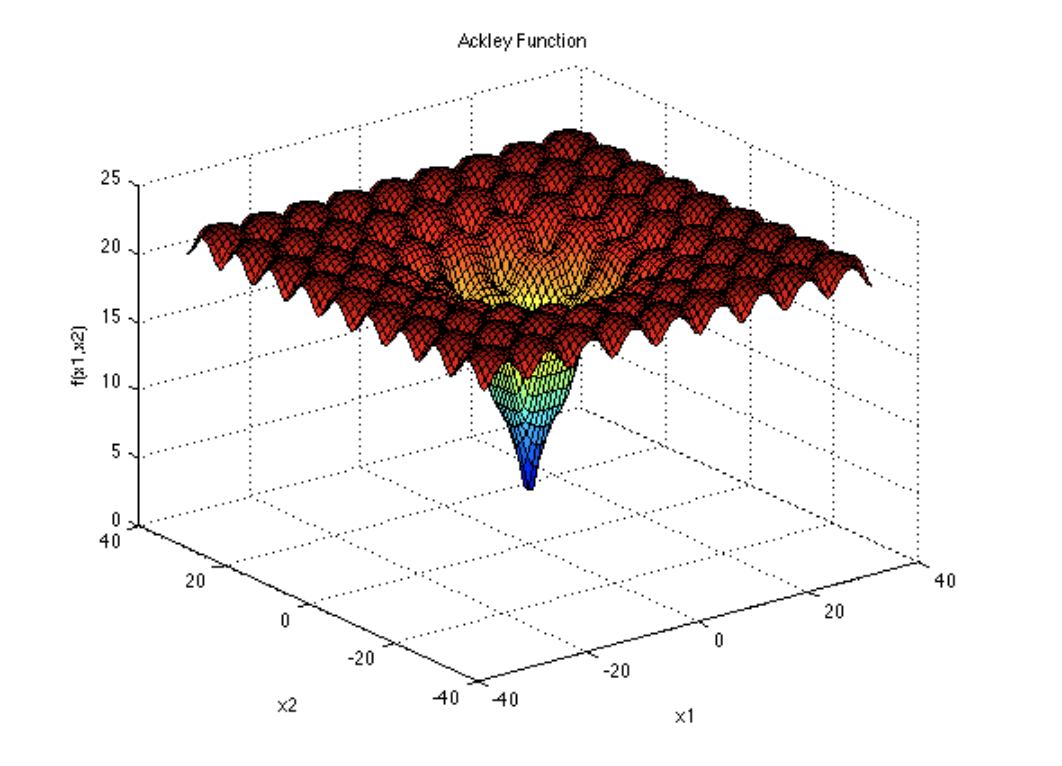
\includegraphics[width=0.8\linewidth]{ackley.png} 
    \caption{Two variable Ackley function. Figure reproduced from \cite{sfu_ackley_nodate}.}
    \label{fig:ackley}
\end{figure}

I added an integration test to \gls{ROLLO} that checks that a default \gls{ROLLO} 
simulation will find the Ackley function's global minimum point. 
If \gls{ROLLO} performed sub-optimally, it would return one of the Ackley 
function's many local minimums. 

\subsection{Binh and Korn Function}
\label{sec:binhandkorn}
The Binh and Korn function \cite{binh_mobes_1997} is a two-objective function:
\begin{align}
    \mbox{Minimize} &= \begin{cases}
        f_1 (x_1,x_2) &= 4x_1^2+4x_2^2 \\
        f_2 (x_1,x_2) &= (x_1-5)^2 + (x_2-5)^2 
    \end{cases} \\
    \mbox{Such that} &= \begin{cases}
        (x_1-8)^2 + (x_2+3)^2 \geq 7.7 \nonumber \\
        0 \leq x_1 \leq 5, 0 \leq x_2 \leq 3 \nonumber
    \end{cases}
\end{align}
We use it as a performance test for multiobjective optimization.
% todo: why is this a good problem? what makes it a good evaluator. 
Figure \ref{fig:binh_paretofront} shows the Binh and Korn function's Pareto front.
\begin{figure}[htbp]
    \centering
    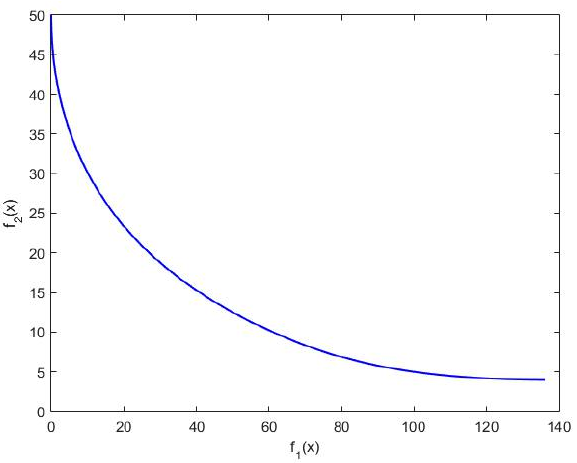
\includegraphics[width=0.7\linewidth]{binh-paretofront.png} 
    \caption{Pareto front of the Binh and Korn test function. Figure reproduced from 
    \cite{bassi_statistics_2018}. }
    \label{fig:binh_paretofront}
\end{figure}
I use the hypervolume indicator to quantify the Pareto front's quality. 
The hypervolume indicator is the most used set-quality indicator for assessing 
stochastic multiobjective optimizers \cite{guerreiro_hypervolume_2020}.
The hypervolume indicator measures the volume (in the objective space) covered by 
non-dominated solutions for problems in which all objectives are to be 
minimized \cite{deb_multi-objective_2001}. 
% todo: remind us of how the reference point is chosen and how it affects hypervolume. 
Figure \ref{fig:pareto_hypervolume} illustrates the hypervolume enclosed by the 
non-dominated solutions (A, B, C, D, E) and reference point, W, in the hatched region 
for a two-dimensional problem.
\begin{figure}[htbp]
    \centering
    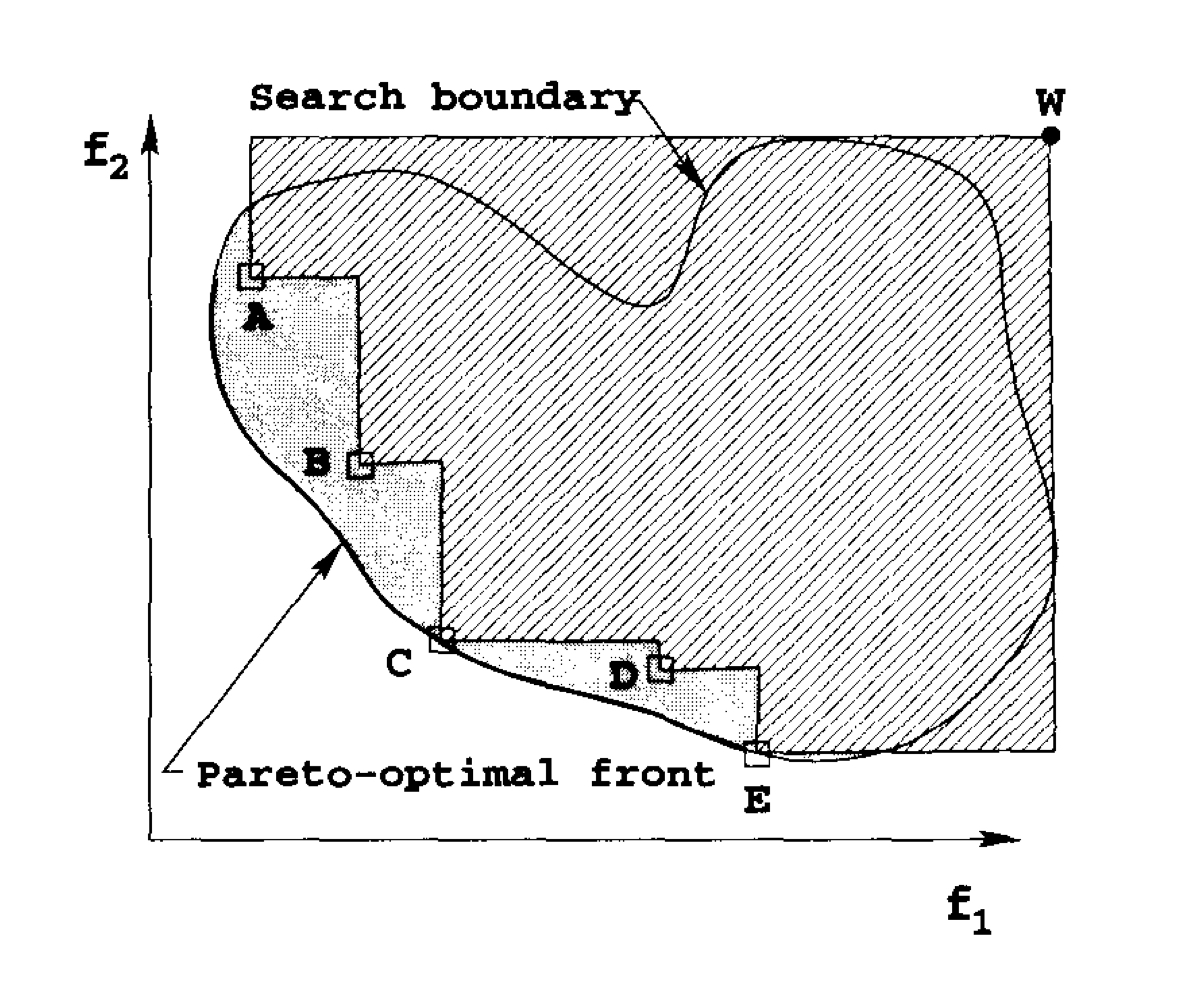
\includegraphics[width=0.7\linewidth]{pareto-hypervolume.png} 
    \caption{Example hypervolume enclosed by non-dominated solutions. Figure reproduced 
    from \cite{deb_multi-objective_2001}. 
    The f1 and f2 axes correspond to the optimization objectives in a \gls{ROLLO} 
    simulation. }
    \label{fig:pareto_hypervolume}
\end{figure}
I added an integration test to ROLLO that checks that a ROLLO simulation will 
find a hypervolume comparable to the ideal Pareto front when minimizing the
Binh and Korn function. 

\subsection{Pu-239 Critical Bare Sphere}
I ran a neutronics verification problem: finding the critical radius for a $^{239}Pu$ 
bare sphere, to ensure successful coupling between \gls{ROLLO} and reactor neutronics 
modeling software, OpenMC \cite{romano_openmc:_2015}. 
The solution to this problem is well studied and readily available in the 
literature \cite{blanchard_updated_1999}. 
Blanchard et al reported that with MCNP4b code and ENDF/B-VI data library, the 
critical mass of a Pu239 bare sphere is 10.00 kg which corresponds to a diameter 
of 9.9cm \cite{blanchard_updated_1999}.
Figure \ref{fig:verification-sphere} shows the ROLLO input file for this verification 
problem. 
In the input file, I vary the radius between 1.0 and 8.0cm, with the objective of 
minimizing the radius while constraining the problem to have $k_{eff} >= 1.0$.
\begin{figure}[htbp]
    \begin{minted}[
        frame=lines,
        framesep=2mm,
        baselinestretch=1.2,
        fontsize=\footnotesize,
        linenos
        ]{json}
        {"control_variables": {
                "radius": {"min": 1.0, "max": 8.0}
            },
            "evaluators": {
                "openmc": {
                    "order": 0,
                    "input_script": ["python", "critical_sphere.py"],
                    "inputs": ["radius"],
                    "outputs": ["keff", "radius"],
                    "output_script": ["python", "get_sphere_keff.py"]
                }
            },
            "constraints": {"keff": {"operator": [">="], 
                            "constrained_val": [1.0]}},
            "algorithm": {
                "parallel": "multiprocessing",
                "keep_files": "none",
                "objective": ["min"],
                "optimized_variable": ["radius"],
                "pop_size": 80,
                "generations": 10
            }}
    \end{minted}
    \caption{\acrfull{ROLLO} JSON input file for finding the minimum radius for 
    a $^{239}Pu$ Critical Bare Sphere.}
    \label{fig:verification-sphere}
\end{figure}
\pagebreak
Figure \ref{fig:critical_sphere.py} shows the OpenMC template used in the 
\gls{ROLLO} simulation. 
\begin{figure}[htbp]
    \begin{minted}[
        frame=lines,
        framesep=2mm,
        baselinestretch=1.2,
        fontsize=\footnotesize,
        linenos
        ]{python}
            import openmc 
            import numpy as np

            pu = openmc.Material()
            pu.set_density("g/cm3", 19.84)
            pu.add_nuclide("Pu239", 1)
            mats = openmc.Materials([pu])
            
            radius = {{radius}}
            
            fuel_sphere = openmc.Sphere(r=radius, boundary_type='vacuum')
            fuel_cell = openmc.Cell(fill=pu, region=-fuel_sphere)
            univ = openmc.Universe(cells=[fuel_cell])
            geom = openmc.Geometry(univ)
            
            settings = openmc.Settings()
            settings.batches = 100
            settings.inactive = 20
            settings.particles = 20000
            settings.temperature = {"multipole": True, "method": "interpolation"}
            
            mats.export_to_xml()
            geom.export_to_xml()
            settings.export_to_xml()
            openmc.run()
    \end{minted}
    \caption{OpenMC template input file used in ROLLO simulation to find the 
    minimum radius for a $^{239}Pu$ Critical Bare Sphere.}
    \label{fig:critical_sphere.py}
\end{figure}  

\gls{ROLLO} successfully finds the critical radius of the $^{239}Pu$ bare sphere 
to be 4.9856cm which corresponds to approximately a 9.9cm diameter. 
The critical sphere's $k_{eff}$ value is 1.00919 $\pm$ 0.00048. 
Figure \ref{fig:verification-radius} and \ref{fig:verification-keff} show the 
radius and $k_{eff}$ evolution through the evolutionary algorithm's 
generations. 
They demonstrate how the average radius converges towards the critical radius while 
constraining $k_{eff} \geq 1$ and improving with each generation.
\begin{figure}[htbp]
    \centering
    \begin{subfigure}{\textwidth}
    \makebox[\textwidth][c]{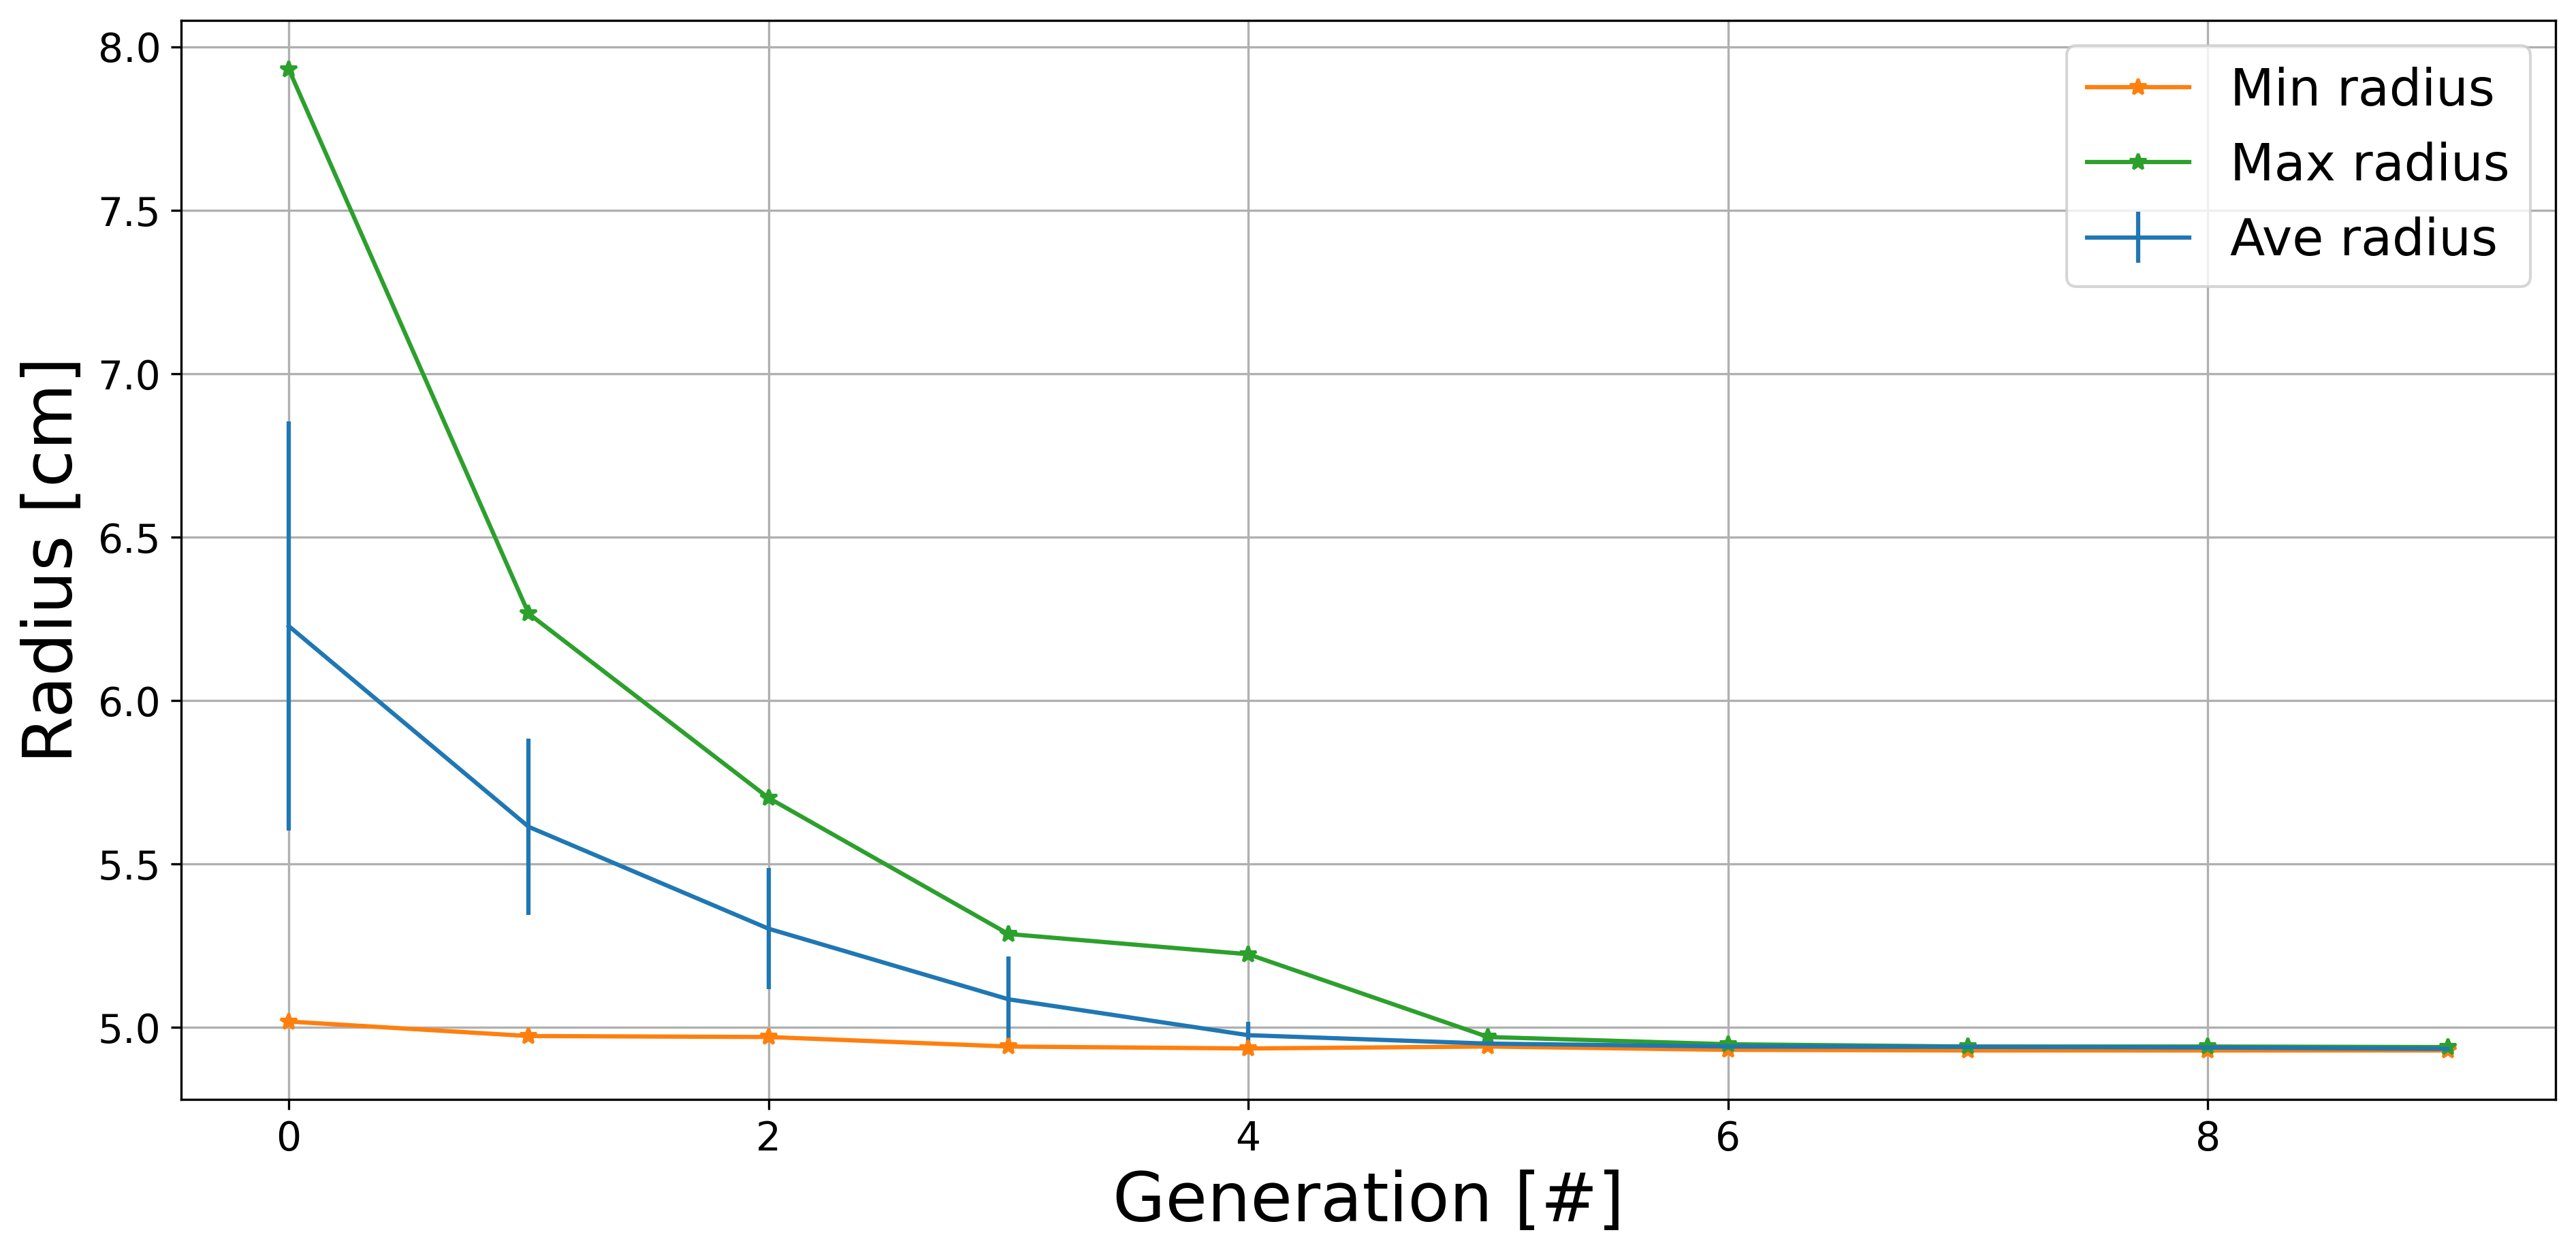
\includegraphics[width=1.1\linewidth]{radius-convergence.png}} 
    \caption{Minimum, average, and maximum radius values evolution.}
    \label{fig:verification-radius}
    \end{subfigure}
    \begin{subfigure}{\textwidth}
        \makebox[\textwidth][c]{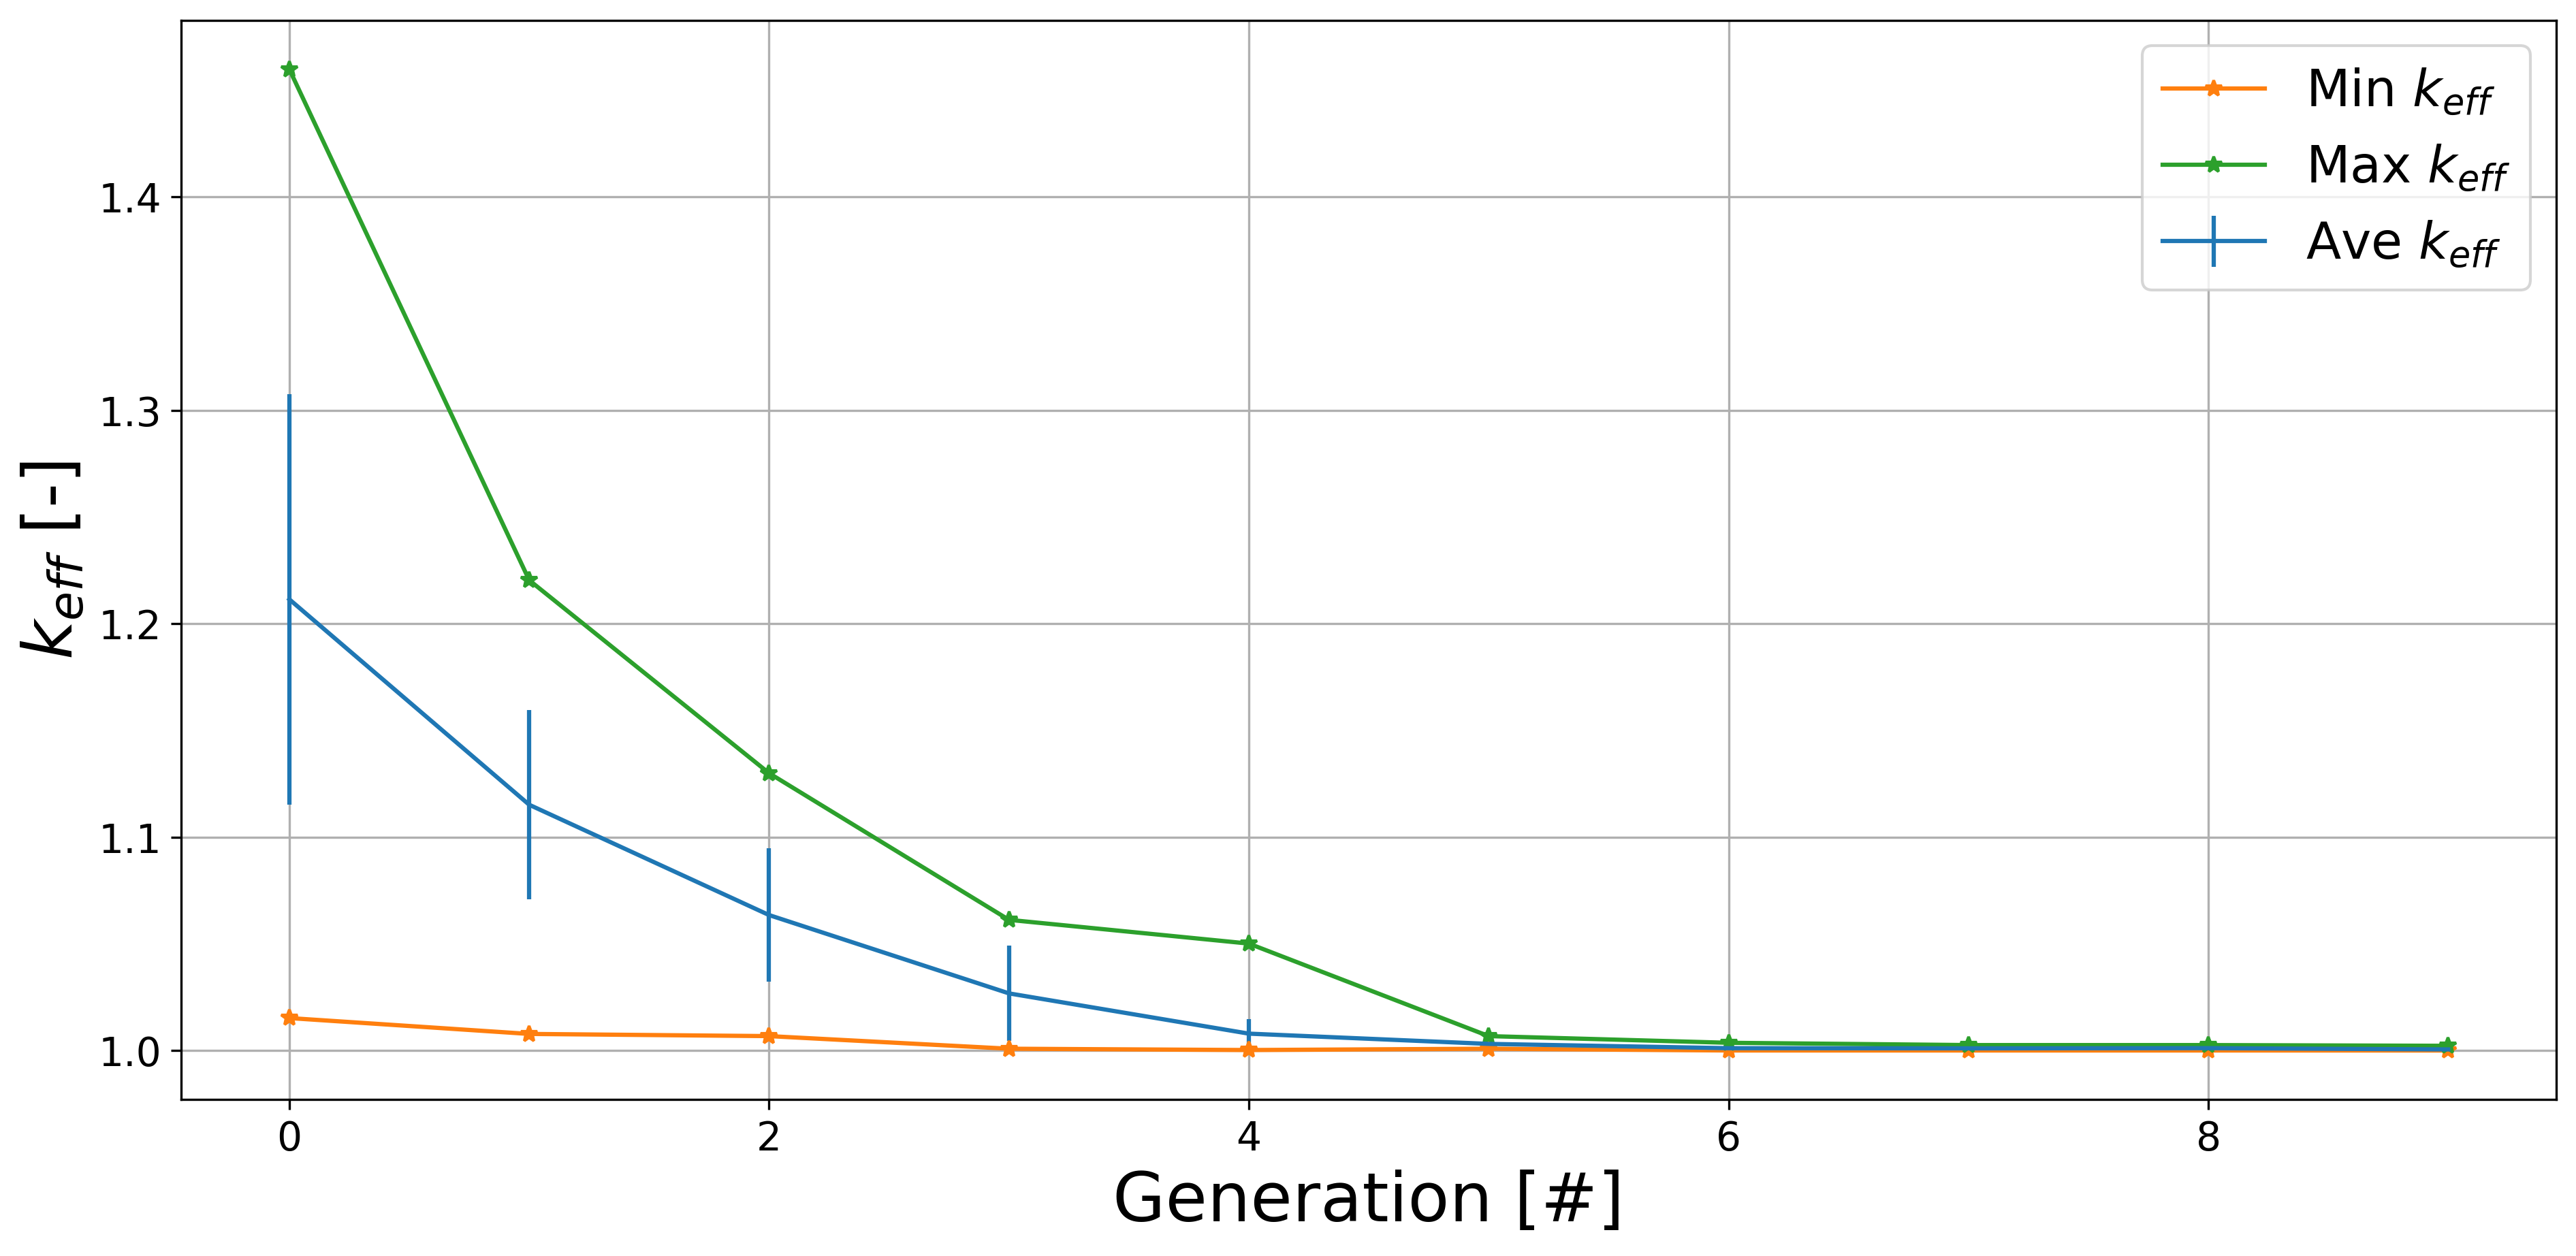
\includegraphics[width=1.1\linewidth]{keff-convergence.png}}
        \caption{Minimum, average, and maximum $k_{eff}$ values evolution.}
        \label{fig:verification-keff}
    \end{subfigure}
    \caption{Results for each generation for \gls{ROLLO}'s genetic algorithm optimization 
    to the find the critical radius of a  $^{239}Pu$ bare sphere.}
\end{figure}

\section{ROLLO Convergence Criteria}
The \texttt{generations} input parameter defines \gls{ROLLO}'s evolutionary algorithm 
convergence criterion. 
Each nuclear reactor model's evaluation is computationally intensive. 
Users will most likely be constrained by the total available compute time. 
Therefore, rather than setting a results-based stopping criterion, ROLLO enables 
users to define the \texttt{generations} and \texttt{pop$\_$size} based on the 
amount of compute time available to them: 
\begin{align}
    t_{total} &= t_{eval} \times gen \times pop 
\intertext{where}
    t_{total} &= \mbox{Total compute time available} \nonumber \\
    t_{eval} &= \mbox{compute time per nuclear reactor model evaluation} \nonumber \\
    gen &= \mbox{total number of generations in optimization process} \nonumber \\
    pop &= \mbox{population size in optimization process} \nonumber
\end{align} 

\subsection{Convergence}
\label{sec:rollo-convergence}
ROLLO does not utilize a mathematical expression to evaluate problem convergence. 
The complexity of reactor design optimization means that no single indicator determines 
if convergence is met.
Instead, ROLLO's purpose is to help the human reactor designer narrow down the design 
space. 
When a ROLLO run completes, the user plots the objectives' convergence and 
Pareto front (for multiobjective simulations) to evaluate if they are confident 
about the final solution set. 
Section \ref{sec:opt} described that an ideal optimization method for a 
multi-objective problem like reactor design should find widely spread solutions 
on the obtained Pareto front \cite{deb_multi-objective_2001}. 
If the simulation is not converged, the user can easily restart the optimization 
simulation using the \texttt{checkpoint.pkl} file and run the problem for a few more 
generations. 
% add about hypervolume for multiobj and obj convergence for singleobj

\section{Summary}
This chapter described the \acrfull{ROLLO} framework developed for 
this dissertation. 
\gls{ROLLO} is a Python package that applies evolutionary algorithm 
optimization techniques to nuclear reactor design using the \acrfull{DEAP} 
module. 
The motivation for \gls{ROLLO} is to enable reactor designers to utilize 
robust evolutionary algorithm optimization methods without going 
through the cumbersome process of setting up a genetic algorithm framework,
selecting appropriate hyperparameters, and setting up its parallelization. 
I designed \gls{ROLLO} to be effective, flexible, open-source, parallel, 
reproducible, and usable. 
\gls{ROLLO} is hosted on Github \cite{chee_rollo_2021}. 